\documentclass[../analysisII_notes.tex]{subfiles}
\begin{document}
\section{Aula 25 - 16 de Junho, 2025}
\subsection{Motivações}
\begin{itemize}
	\item Vetor Tangente/Velocidade;
	\item Vetor Gradiente;
\end{itemize}
\subsection{Interpretações Geométricas da Derivada.}
O objetivo dessa aula é justamente dar mais conteúdo geométrico ao conceito de uma aplicação entre espaços euclidianos. Primeiramente, faremos isto construindo a noção do \textit{vetor tangente}, ou \textit{velocidade}, de uma curva.
\begin{def*}
	Um \textbf{caminho em }\(\mathbb{R}^{n}\) é uma aplicação contínua \(\gamma :I\rightarrow \mathbb{R}^{n}\) definida num intervalo I qualquer da reta real. Se, além disso, \(\gamma(I)\) é um subconjunto de \(U\subseteq \mathbb{R}^{n},\) diremos que é um \textbf{caminho em U}. \(\square\)
\end{def*}
\begin{figure}[H]
	\begin{center}
		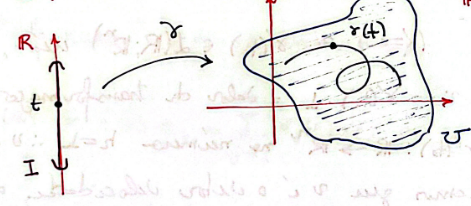
\includegraphics[height=\textheight, width=\textwidth, keepaspectratio]{./Images/paths_25.png}
	\end{center}
	\caption{a função \(\gamma \) mapeia o intervalo continuamente em \(\mathbb{R}^{n}\).}
\end{figure}
conforme vimos previamente, esta curva \(\gamma \) com as mesmas notações da definição se escreve em termos de suas n coordenadas:
\[
	\gamma_1,\dotsc ,\gamma_{n}:I\rightarrow \mathbb{R} \Rightarrow \gamma(t) = (\gamma_1(t), \gamma_2(t), \dotsc ,\gamma_{n}(t)),\; t\in I.
\]
\begin{def*}
	Diremos que um caminho \(\gamma \) possui um \textbf{vetor velocidade no ponto }\(t_{0}\) de I quando existir um vetor \(v\in \mathbb{R}^{n}\) tal que
	\[
		v = \lim_{t\to t_{0}}\frac{\gamma(t)-\gamma(t_{0})}{t-t_{0}} = \lim_{h\to 0}\frac{\gamma(t_{0}+h) - \gamma(t_{0})}{h}.
	\]
	Neste caso, escrevemos
	\[
		v = \frac{\mathrm{d}\gamma }{\mathrm{d}t}(t_{0}) = \biggl(\frac{\mathrm{d}\gamma_1}{\mathrm{d}t}(t_{0}), \dotsc , \frac{\mathrm{d}\gamma_{n}}{\mathrm{d}t}(t_{0})\biggr),
	\]
	e o chamamos \textbf{vetor velocidade de }\(\gamma \)\textbf{ em }\(t_{0}.\; \square\)
\end{def*}
\begin{figure}[H]
	\begin{center}
		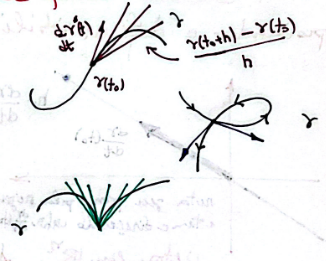
\includegraphics[height=0.5\textheight, width=0.5\textwidth, keepaspectratio]{./Images/tangent_vectors_25.png}
	\end{center}
	\caption{vetores tangentes a diferentes formatos de caminhos}
\end{figure}

\begin{tcolorbox}[
		skin=enhanced,
		title=Observação,
		fonttitle=\bfseries,
		colframe=black,
		colbacktitle=cyan!75!white,
		colback=cyan!15,
		colbacklower=black,
		coltitle=black,
		drop fuzzy shadow,
		%drop large lifted shadow
	]
	Quando \(\frac{\mathrm{d}\gamma }{\mathrm{d}t}(t_{0})\) é diferente de 0, alguns afuroes costumam chamá-lo de \textbf{vetor tangente em }\(t_{0}\), não em \(\gamma(t_{0})\), e estaremos adotando esta notação.
\end{tcolorbox}
\begin{prop*}
	Dado que I é um aberto, um caminho \(\gamma :I\rightarrow \mathbb{R}^{n}\) possui vetor velocidade em \(t_{0}\) se, e somente se, \(\gamma \) é diferenciável em \(t_{0}\). Em caso afirmativo,
	\[
		\gamma'(t_{0})\cdot h = h \cdot \frac{\mathrm{d}\gamma }{\mathrm{d}t}(t_{0}),\quad h\in \mathbb{R}.
	\]
\end{prop*}
\begin{figure}[H]
	\begin{center}
		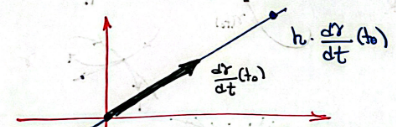
\includegraphics[height=0.5\textheight, width=0.5\textwidth, keepaspectratio]{./Images/directed_velocity_25.png}
	\end{center}
	\caption{reta que passa pela origem e tem direnção do vetor \(\frac{\mathrm{d}\gamma }{\mathrm{d}t}(t_{0})\).}
\end{figure}

\begin{proof*}
	\(\Rightarrow )\) Escrevendo, para h positivo,
	\[
		r(h) = \gamma(t_{0}+h) - \gamma(t_{0}) - h \cdot \frac{\mathrm{d}\gamma(t_{0})}{\mathrm{d}t},
	\]
	segue que
	\[
		\frac{r(h)}{|h|} = \frac{\gamma(t_{0}+h) - \gamma(t_{0})}{h} - \frac{\mathrm{d}\gamma (t_{0})}{\mathrm{d}h}\overbracket[0pt]{\longrightarrow}^{h\to 0^{+}}0;
	\]
	analogamente, se h for negativo, tem-se
	\[
		\frac{r(h)}{|h|} =\frac{\gamma(t_{0}+h) - \gamma(t_{0}) }{-h} + \frac{\mathrm{d}\gamma(t_{0})}{\mathrm{d}t} = \frac{\mathrm{d}\gamma(t_{0})}{\mathrm{d}t} -\biggl[\frac{\gamma(t_{0}+h)-\gamma(t_{0})}{h}\biggr]\overbracket[0pt]{\rightarrow}^{h\to 0^{-}}0,
	\]
	provando a diferenciabilidade de \(\gamma \) em \(t_{0}\), com
	\[
		\gamma'(t_{0})\cdot h = h \cdot \frac{\mathrm{d}\gamma }{\mathrm{d}t}(t_{0})
	\]

	\(\Leftarrow )\) Se \(\gamma'(t_{0})\) é uma aplicação linear de \(\mathbb{R}\) em \(\mathbb{R}^{n}\), seja v o valor da transformação linear \(\gamma'(t_{0}):\mathbb{R}\rightarrow \mathbb{R}^{n}\) no número \(h=1\), ou seja,
	\[
		v\coloneqq \gamma'(t_{0})\cdot 1.
	\]
	Assim, v é um vetor em \(\mathbb{R}^{n}\), e afirmamos que ele é de fato o vetor velocidade de \(\gamma \) em \(t_{0}\).

	Com efeito,
	\begin{align*}
		\lim_{h\to 0}\biggl[\frac{\gamma(t_{0}+h) - \gamma(t_{0})}{h}\biggr] & = \lim_{h\to 0}\biggl[\frac{\gamma(t_{0}+h)-\gamma(t_{0})-\gamma'(t_{0})\cdot h}{h}\biggr]         \\
		                                                                     & = \lim_{h\to 0}\biggl[\frac{\gamma(t_{0}+h) - \gamma(t_{0}) -\gamma'(t_{0})\cdot h}{\pm|h|}\biggr] \\
		                                                                     & = \pm\lim_{h\to 0}\frac{r(h)}{|h|}=0.\quad \text{\qedsymbol}
	\end{align*}
\end{proof*}

O segundo elemento que vamos estudar é o \textit{vetor gradiente} de uma função  a valores reais definida num aberto U de \(\mathbb{R}^{m}\), ou seja, \(f:U\subseteq \mathbb{R}^{m}\rightarrow \mathbb{R}\).

\begin{def*}
	Quando f é diferenciável num ponto a do aberto U, definimos o \textbf{gradiente de f em a} como
	\[
		\nabla f(a) = \biggl(\frac{\partial^{}f}{\partial x_1^{}}(a), \frac{\partial^{}f}{\partial x_2^{}}(a), \dotsc , \frac{\partial^{}f}{\partial x_{m}^{}}(a)\biggr). \;\square
	\]
\end{def*}
Para entender como o gradiente de f se relaciona com sua derivada em a, faremos uso da ajuda da base canônica de \(\mathbb{R}^{m}\), denotada por
\[
	\mathcal{B}=\{e_1, e_2, \dotsc , e_{m}\},\quad e_{j} = (\delta_{ij}).
\]
Associada a esta base \(\mathcal{B}\), está a sua \textbf{base dual} em \((\mathbb{R}^{m})^* = \mathcal{L}(\mathbb{R}^{m}; \mathbb{R})\), indicada e definida respectivamente por
\begin{align*}
	 & (I)\; \mathcal{B}^*\coloneqq \{dx_1, dx_2, \dotsc , dx_{m}\},\quad dx_{i}\cdot e_{j} = \delta_{ij},\; 1\leq i, j\leq m; \\
	 & (II)\; dx_{i}\cdot u = u_{i},\quad u = (u_1, u_2, \dotsc , u_{m})\in \mathbb{R}^{m},\; i = 1, 2, \dotsc , m.
\end{align*}

Em cada ponto a de u, a derivada \(f'(a)\) pertence ao dual de \(\mathbb{R}^{m}\), ou seja, \(f'(a)\in (\mathbb{R}^{m})^*\), donde segue que existe escalares \(\alpha_1(a),\dotsc ,\alpha_{m}(a)\) reais, tais que
\[
	f'(a) = \alpha_1(a)dx_1 + \dotsc \alpha_{m}(a)dx_{m},
\]
e as definições das ``diferenciais'' e das derivadas parciais nos dão, indiretamente,
\[
	\frac{\partial^{}f}{\partial x_{i}^{}}(a) = f(a)\cdot e_{i} = \sum\limits_{j=1}^{m}\alpha_{j}(a)dx_{j}\cdot e_{i} = \alpha_{i}(a),\; i = 1, 2, \dotsc , m.
\]
Com isso, podemos definir
\begin{def*}
	O \textbf{diferencial de f em a}, denotado por \(df(a)\), é o objeto
	\[
		df(a) = \sum\limits_{j=1}^{m}\frac{\partial^{}f}{\partial x_{j}^{}}(a)dx_{j}
	\]
	escrito explicitamente como
	\[
		f'(a) = \frac{\partial^{}f}{\partial x_1^{}}(a)dx_1 + \dotsc + \frac{\partial^{}f}{\partial x_{m}^{}}(a)dx_{m}. \quad \square
	\]
\end{def*}
Assim, unindo o clássico ao moderno,
\[
	f'(a) = df(a).
\]
Logo, em cada elemento a de U,
\[
	\nabla f(a) = \biggl(\frac{\partial^{}f}{\partial x_1^{}}(a),\dotsc , \frac{\partial^{}f}{\partial x_{m}^{}}(a)\biggr)
\]
é o vetor de \( \mathbb{R}^{m}\) cujas coordenadas na base canônica \(\mathcal{B}\) de \(\mathbb{R}^{m}\) são as coordenadas da derivada \(f'(a) = df(a)\) na base canônica dual \(\mathcal{B}^* \) de \((\mathbb{R}^{m})^{*}\).

Com isso, um problema analisado melhor na área da geometria diferencial é justamente entender como mudam as coordenadas de \(df(a)\) ao mudarmos as coordenadas de \(\mathbb{R}^{m} = T_{a}U\) para cada ponto a de U.
\begin{tcolorbox}[
		skin=enhanced,
		title=Observação,
		fonttitle=\bfseries,
		colframe=black,
		colbacktitle=cyan!75!white,
		colback=cyan!15,
		colbacklower=black,
		coltitle=black,
		drop fuzzy shadow,
		%drop large lifted shadow
	]
	Nessa mesma ordem de ideias, dado um vetor \(h=(h_1, \dotsc , h_{m})\) de \(\mathbb{R}^{m}\), obtivemos uma regra explícita para calcular a derivada direcional de f na direção de h! Especificamente,
	\[
		f'(a)\cdot h = \sum\limits_{j=1}^{n}\frac{\partial^{}f}{\partial x_{j}^{}}(a)\cdot dx_{j}\cdot h = \sum\limits_{j=1}^{m}\frac{\partial^{}f}{\partial x_{j}^{}}(a)\cdot h_{j} = \left< \nabla f(a), h \right>.
	\]
	Na notação de derivadas direcionais, a igualdade acima fica
	\[
		\frac{\partial^{}f}{\partial h^{}}(a) = \left< \nabla f(a), h \right>,
	\]
\end{tcolorbox}

Agora, podemos entender o papel do vetor velocidade do gradiente no estudo do comportamento local de uma função real definida num aberto de \(\mathbb{R}^{m}.\) Fixado a em U, considere o caminho retilíneo \(\lambda :(-\varepsilon , \varepsilon )\rightarrow U\) dado por
\[
	\lambda (t)=a+t \cdot h,\quad h\in \mathbb{R}^{m},
\]
onde \(\varepsilon \) é um valor positivo e escolhido para que, se \(|t|<\varepsilon \), então \(a+th\) pertence a U (é possível por U ser aberto). Assim, f transforma o caminho \(\lambda(t)=a+t \cdot h\) no caminho \(\varphi (t)=f(a+th)\):
\begin{figure}[H]
	\begin{center}
		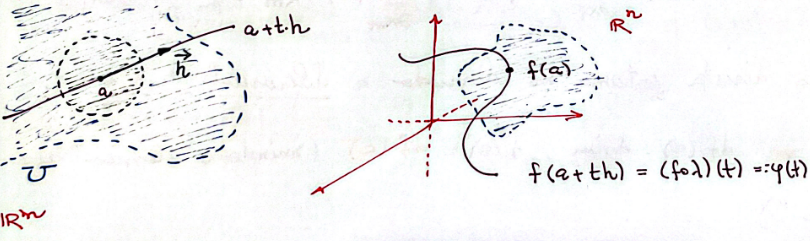
\includegraphics[height=0.8\textheight, width=0.8\textwidth, keepaspectratio]{./Images/f_to_phi_25.png}
	\end{center}
	\caption{a função f transforma o caminho \(\lambda \) no caminho \(\varphi (t)\).}
\end{figure}
Tanto no caso geral de \(f:\mathbb{R}^{m}\rightarrow \mathbb{R}^{n}\) quanto no caso \(f:\mathbb{R}^{m}\rightarrow \mathbb{R}\), a função \(\varphi:J\rightarrow \mathbb{R} \) é uma função real de uma variável real que, usando as definições e identificações que fizemos até agora, dá
\[
	\frac{\mathrm{d}\pi }{\mathrm{d}t}(0) = \lim_{t\to 0}\frac{\varphi (t)-\varphi (0)}{t} = \lim_{t\to 0}\frac{f(a+th)-f(a)}{t} = \frac{\partial^{}f}{\partial h^{}}(a)=f'(a)\cdot h,
\]
ou seja, a derivada direcional de f em a na direção de h dá informações sobre o crescimento de \(\varphi \). Mais geralmente, para \(t_{0}\) no intervalo \((-\varepsilon , \varepsilon )\) qualquer, tem-se
\begin{align*}
	\frac{\mathrm{d}\varphi }{\mathrm{d}t}(t_{0}) & = \lim_{t\to 0}\frac{\varphi (t+t_{0})-\varphi(t_{0})}{t}          \\
	                                              & = \lim_{t\to 0}\frac{f(a+(t+t_{0})\cdot h)-f(a+t_{0}\cdot h)}{t}   \\
	                                              & = \lim_{t\to 0}\frac{f([a+t_{0}\cdot h]+th) -f(a+t_{0}\cdot h)}{t} \\
	                                              & = \frac{\partial^{}f}{\partial h^{}}(a+t_{0}\cdot h).
\end{align*}

\begin{prop*}[Propriedades]
	Seja \(f:U\subseteq \mathbb{R}^{m}\rightarrow \mathbb{R}\) uma função diferenciável. Supondo que a é um ponto regular, ou seja, \(\nabla f(a)\neq 0\), valem as propriedades:
	\begin{itemize}
		\item[i)] Dado a um ponto de U, o vetor \(\nabla f(a)\) aponta para uma direção segundo a qual f cresce;
		\item[ii)] Dentre \textit{todas} as direções ao longo das quais f cresce, a do \(\nabla f(a)\) é aquela de crescimento mais rápido; e
		\item[iii)] O vetor \(\nabla f(a)\) é ortogonal à superfície de nível \(f(x) = f(a) = c.\)
	\end{itemize}
\end{prop*}
\begin{proof*}
	A demonstração em si já foi dada de forma fragmentada do longo das discussões, então iremos mais juntar os pedaços do que qualquer outra coisa.

	(i) Pelas observações, sabemos que, dado um ponto \(t_{0}\) em \((-\varepsilon , \varepsilon )\), temos
	\[
		\frac{\mathrm{d}^{}\varphi }{\mathrm{d} t^{}}(t_{0}) = \frac{\partial^{}f}{\partial h^{}} (a+t_{0}\cdot h) = \left< \nabla f(a+t_{0}\cdot h), \nabla f(a) \right>,\; h = \nabla f(a)
	\]
	e, sendo
	\[
		\frac{\mathrm{d}\varphi (0)}{\mathrm{d}t} = |\nabla f(a)|^{2} > 0,
	\]
	podemos escolher \(\varepsilon  > 0\) para o qual
	\[
		|t_{0}| < \varepsilon  \Rightarrow \frac{\mathrm{d}\varphi }{\mathrm{d}t}(t_{0}) > 0,
	\]
	ou seja, para que \(\varphi \) seja uma \textit{função crescente}, que é exatamente o que queríamos provar

	(ii) Se \(w\neq 0\) for uma direção qualquer em \(\mathbb{R}^{m}\), então
	\[
		\frac{\partial^{}f}{\partial w^{}}(a) = \left< \nabla f(a), w \right> \leq |\nabla f(a)|\cdot |w|.
	\]
	Assim, sendo \(|w| = 1\), o que temos é
	\[
		\frac{\partial^{}f}{\partial w^{}}(a) \leq |\nabla f(a)| = \biggl< \nabla f(a), \frac{\nabla f(a)}{|\nabla f(a)|} \biggr>.
	\]
	Logo, a direção de \(\nabla f(a)\) é aquela que dá o maior valor para \(\frac{\partial^{}f}{\partial w^{}}(a)\) dentre todas as possíveis direções w com \(|w|=1\), que é o que queríamos dizer na propriedade (ii).
	\begin{figure}[H]
		\begin{center}
			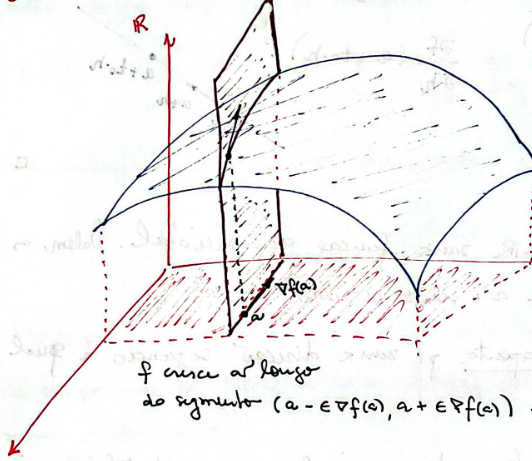
\includegraphics[height=0.5\textheight, width=0.5\textwidth, keepaspectratio]{./Images/growth_f_25.png}
		\end{center}
		\caption{a função f cresce ao longo do segmento \((a-\varepsilon \nabla f(a), a+\varepsilon \nabla f(a))\)}
	\end{figure}

	(iii) Seja, agora, \(\gamma :J\rightarrow U\) um caminho dentro da superfície de nível \(f(x) = f(a)\), ou seja,
	\[
		\{x\in U:\; f(x) = f(a)\} = f^{-1}(x),\quad c = f(a).
	\]
	Isto significa que \(c = f(\gamma (t))\) para qualquer t em J, e que, derivando,
	\[
		0 = \frac{\mathrm{d}}{\mathrm{d}t}(f\circ \gamma )(t) = \left< \nabla f(\gamma (t)),\gamma'(t)  \right>,\quad \forall t\in J,
	\]
	que é legítimo por termos demonstrado a regra da cadeia. Em particular, se \(\gamma (0) = p\), então \(\gamma'(0)\) é o vetor tangente em p, e a igualdade acima se escreve
	\[
		0 = \left< \nabla f(p), \gamma '(0) \right>.
	\]
	\begin{figure}[H]
		\begin{center}
			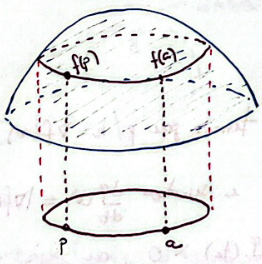
\includegraphics[height=0.4\textheight, width=0.4\textwidth, keepaspectratio]{./Images/level_surface_25.png}
		\end{center}
		\caption{f e sua pré-imagem de pontos em \(f^{-1}(c)\) e fora.}
	\end{figure}

	Portanto, f(a) é ortogonal a \(\gamma '(0)\); isto é, \(\nabla f(a)\perp \gamma '(0)\).
	\begin{figure}[H]
		\begin{center}
			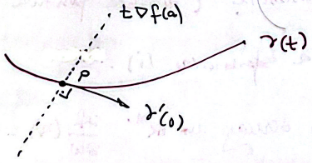
\includegraphics[height=0.5\textheight, width=0.5\textwidth, keepaspectratio]{./Images/orthogonality_25.png}
		\end{center}
		\caption{\(\gamma '(0)\) como ortogonal ao gradiente de f em a.\qedsymbol}
	\end{figure}
\end{proof*}
\end{document}
